\section{Architekturstile}
Die Architektur von Anwendungen in den meisten Fällen als monolithisch oder als Microservice Architektur bezeichnen \cite[Vgl.][S. 150]{Gos2020}. Das nachfolgende Kapitel beschreibt diese Architekturstile mit ihren Eigenschaften und warum die Microservice Architektur für den Betrieb in der Cloud bevorzugt eingesetzt wird \cite[Vgl.][S. 1]{Villamizar2015}.

\subsection{Monolithische Anwendungsarchitektur}
% Was sind monolithishue Anwendungen?
Monolithische Anwendungen, wie sie in der Vergangenheit oft eingesetzt wurden, bestehen aus verschiedenen Komponenten, die zu einem Programm kombiniert werden. Die einzelnen Komponenten funktionieren nur zusammen innerhalb des Programmes \cite[Vgl.][S. 1]{Gos2020}.

\begin{figure}[H]
    \centering
    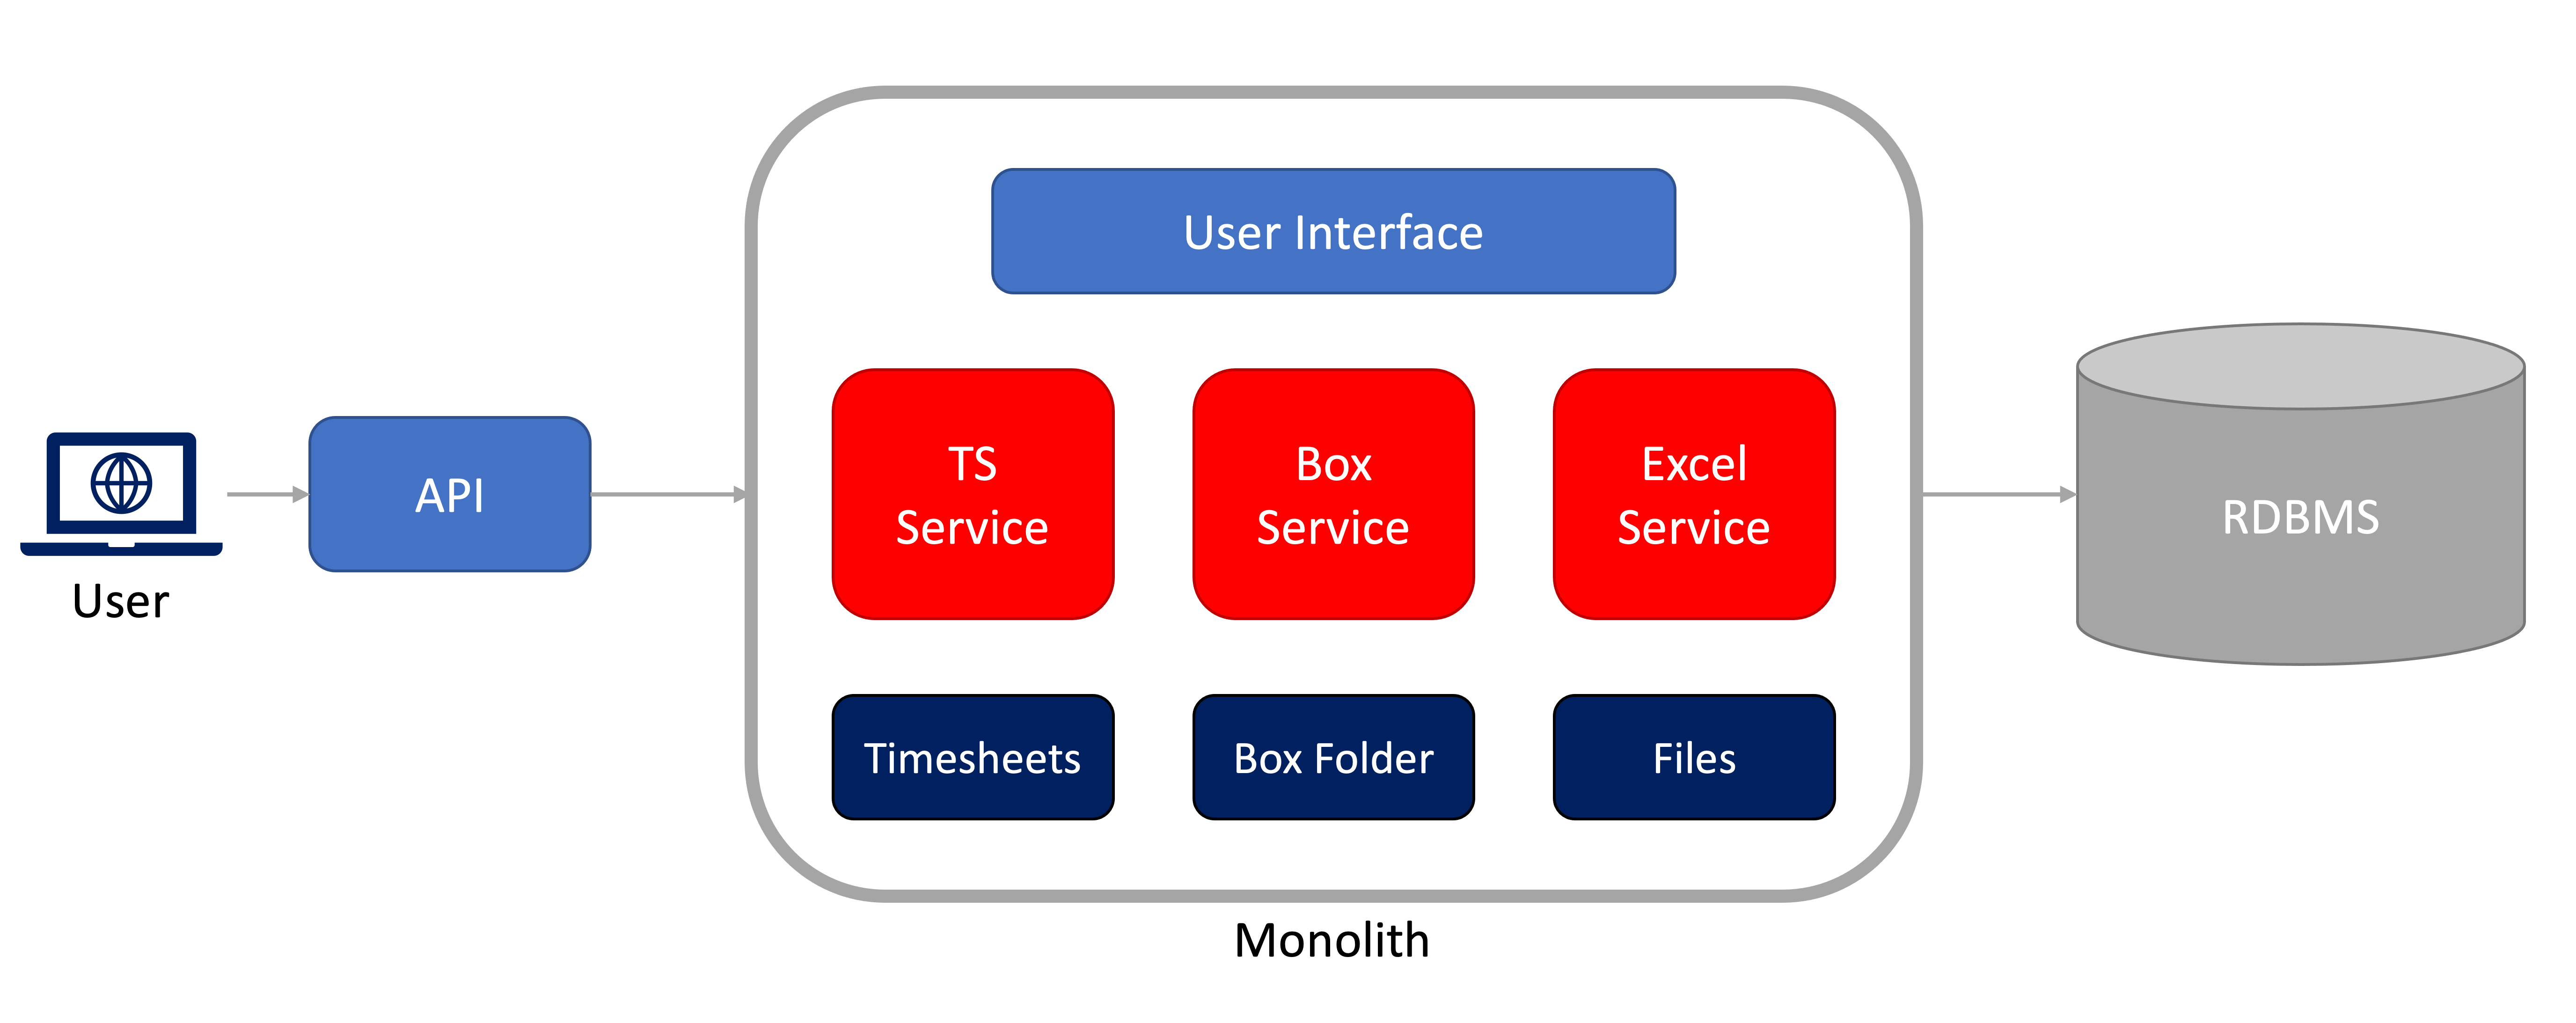
\includegraphics[width=0.65\textwidth]{monolith.png}
    \caption{Beispiel einer monolithischen Architektur \cite[Nachbildung angelehnt an][S. 150]{Gos2020}}
    \label{fig:monolith}
\end{figure}

Abbildung \ref{fig:monolith} zeigt, wie eine monolithische Architektur aufgebaut sein kann, am Beispiel des in dieser Arbeit untersuchten Collect-Services. Hier sind die Komponenten eng miteinander verwoben und voneinander abhängig.
% In Bezug auf Cloud Native -> warum nicht geeignet
\pagebreak

\subsection{Microservice Architektur}

\begin{figure}[H]
    \centering
    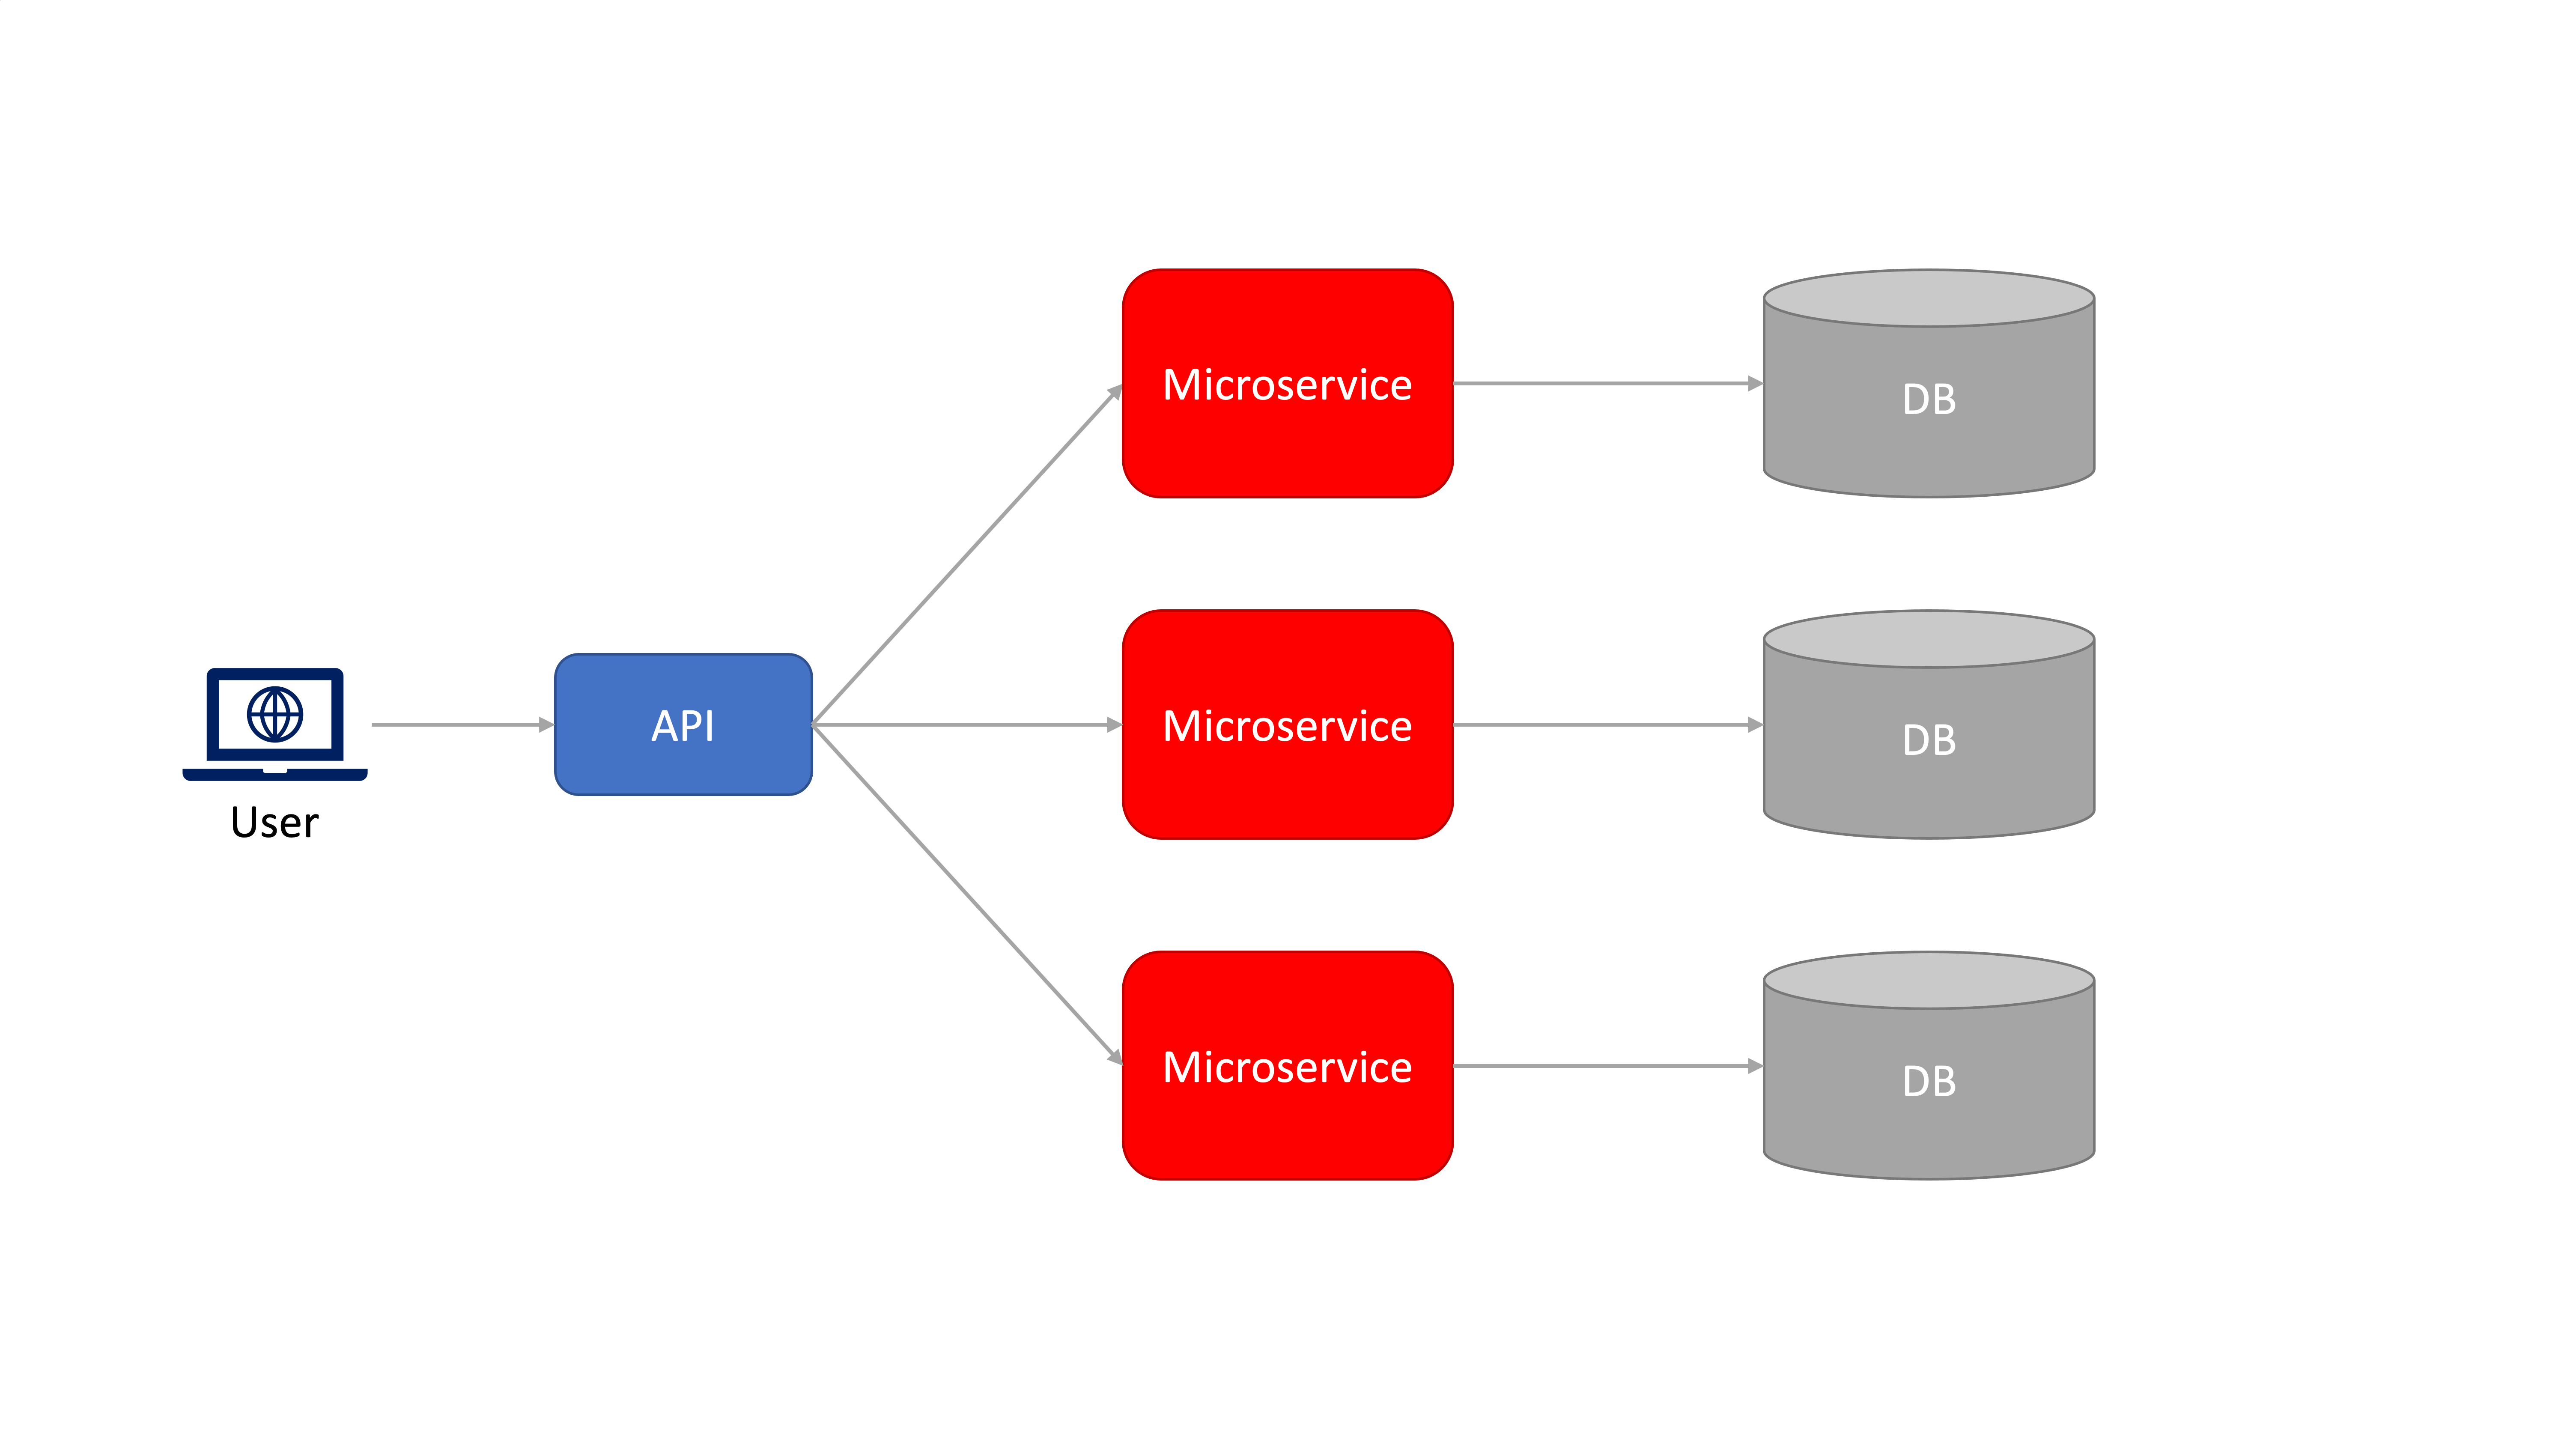
\includegraphics[width=0.65\textwidth]{microservice.png}
    \caption{Beispiel einer Microservice Architektur \cite[Nachbildung angelehnt an][S. 150]{Gos2020}}
    \label{fig:microservice}
\end{figure}

% Wann/Wie